

As the multi-headed attention is logically partitioned, separate weight matrices are used for each head. \\
After the self attention scores have been calculated (\Cref{fig:attention_score_matrix_form}) for each attention head as there are now
eight separate matrices (one for each attention head\footnote{Eight is the default value, although this can be configured.}). The correct shape
must be obtained to satisfy the desired input shape of the feed forward layer. This layer is expecting a single matrix, so the attention heads
matrices are simply concatenated and multiplied with a further weight matrix obtained\footnote{This weight matrix is adjusted during training.} as per
\Cref{fig:concat_atn_head_matrices}. The idea here is to keep the values of the words that are relevant and drown out the irrelevant words by multiplying
them by a small numbers, a typical value would be 0.01. This returns the desired effect.
\begin{figure}[H]
	\centering
	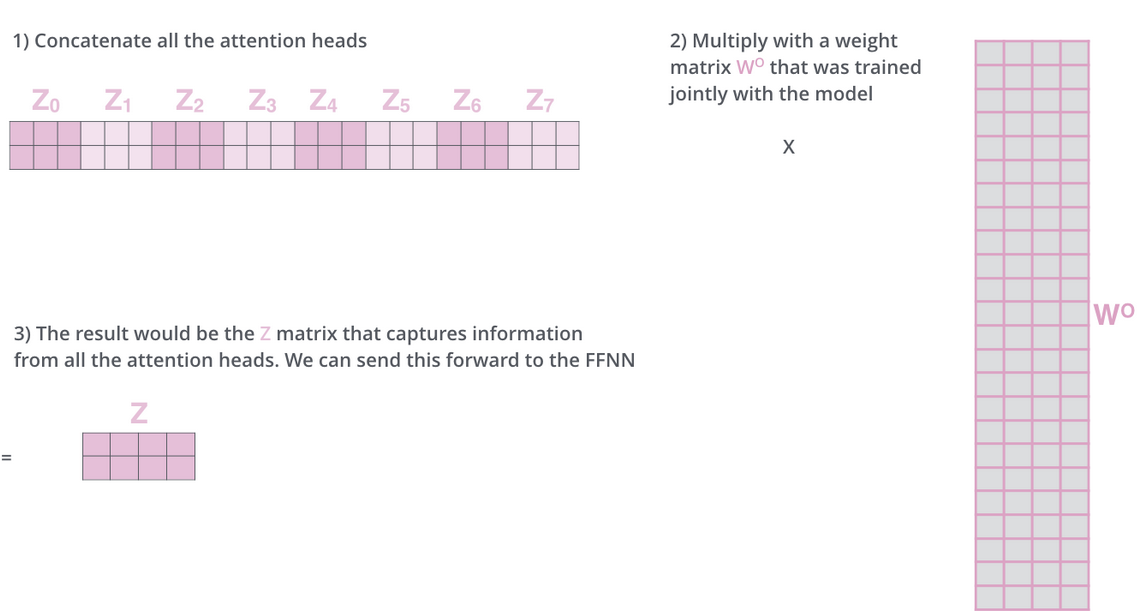
\includegraphics[width=0.9\textwidth]{figures/concat_atn_head_matrices.png}
	\caption{Concatenated Attention Head Matrices as sourced from here~\autocite{alammarIllustratedTransformer}}
	\label{fig:concat_atn_head_matrices}
\end{figure}
\Cref{fig:atn_summary} depicts a way to visualze the entire process. As previously detailed, and can be seen, the embeddings are only
used in the inital pass into the encoder, all subsequent traversals use \code{R}, which is the output of the encoder directly preceding the
current encoder.
\begin{figure}[H]
	\centering
	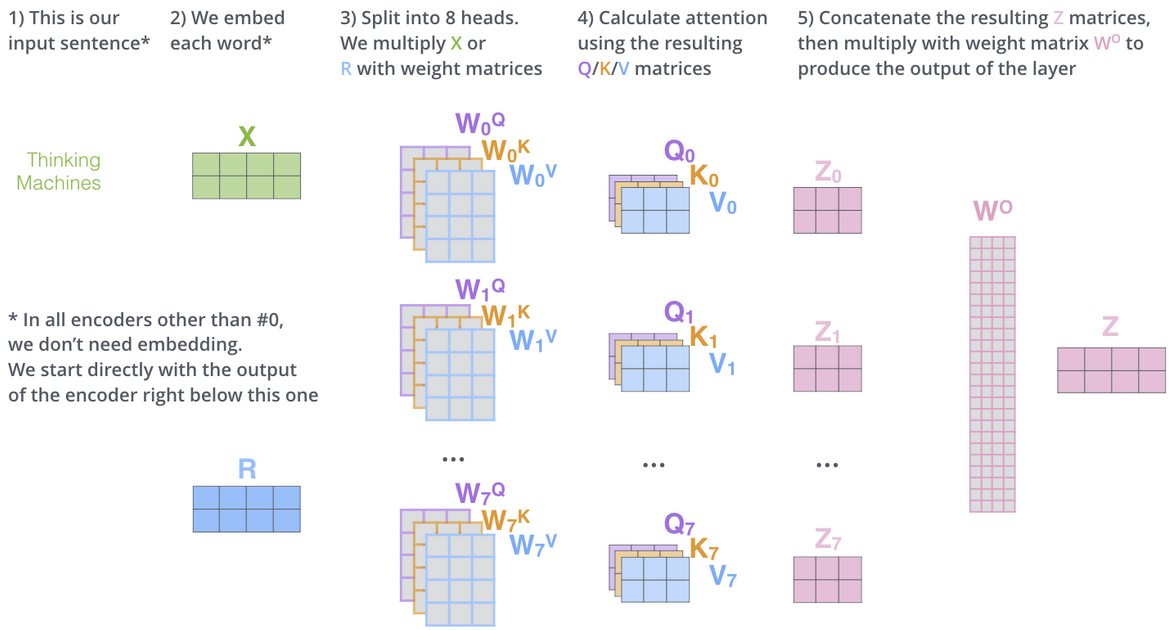
\includegraphics[width=1\textwidth]{figures/atn_summary.png}
	\caption{Attention Summary from here~\autocite{alammarIllustratedTransformer}}
	\label{fig:atn_summary}
\end{figure}
The attention score calculation is carried out in step \textbf{4} as depicted in \Cref{fig:atn_summary}. \\
\subsection{Attention Intuition}
The formula along with its place in the encoder and the inputs have now been detailed, yet it is important to develop an intuition of
why the formula works and how this formula returns useful scores.\\
To do this here is an example starting with the dot product calculation of the Query (Q) and Key (K)\textsuperscript{Transpose} matrices
as per the formula and depicted in \Cref{fig:q_kt_dot_product}. Lets call this the `factor matrix'.
\begin{figure}[H]
	\centering
	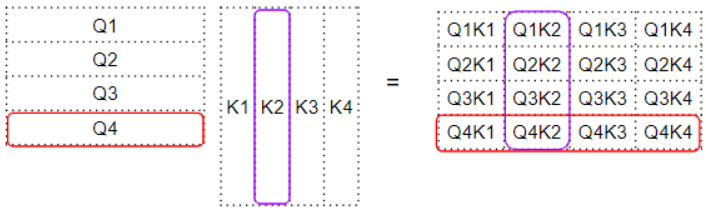
\includegraphics[width=0.7\textwidth]{figures/dot_prodct_q_kt.png}
	\caption{Dot Product of Query and Key Transpose sourced from here~\autocite{doshiTransformersExplainedVisually2021b}}
	\label{fig:q_kt_dot_product}
\end{figure}
Other calculations the division and square root of the formula are not shown here, as they do not alter the matrix but merely configure its
shape and manipulate it so that the score can be calculated more easily.
\bigbreak
Now that the dot product of (QK\textsuperscript{T}), the next part of the formula is to obtain the
dot product of the result of (QK\textsuperscript{T})\footnote{Query Key\textsuperscript{T}} with the V or Values matrix as per \Cref{fig:qk_v_dot_product}.
\begin{figure}[H]
	\centering
	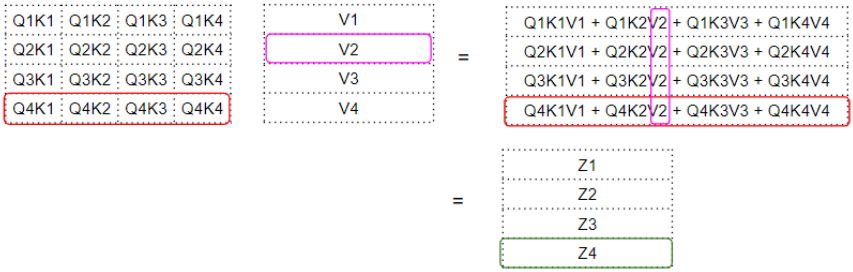
\includegraphics[width=1\textwidth]{figures/qk_v_dot_product.png}
	\caption{Dot Product of Query Key Transpose and Values sourced from here~\autocite{doshiTransformersExplainedVisually2021b}, depicting the
		resulting attention score.}
	\label{fig:qk_v_dot_product}
\end{figure}
Z is the resulting attention score vector. A way to understand the sequence of events is to think about the ouput score.
For each word, the attention score is the encoded value of every word from the `Value' matrix, weighted by the `factor'
matrix. The factor matrix itself is the dot product of the Query value for the specified word with the Key value of all
words as\autocite{doshiTransformersExplainedVisually2021b} per \Cref{fig:atn_weight_summation}.
\begin{figure}[H]
	\centering
	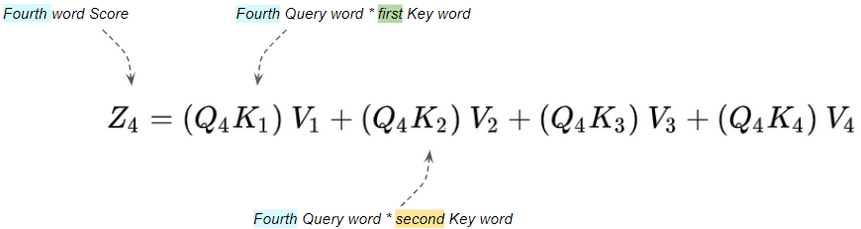
\includegraphics[width=0.9\textwidth]{figures/atn_weight_summation.png}
	\caption{Attention Weight Summation from here~\autocite{doshiTransformersExplainedVisually2021b}, depicting the resulting attention score.}
	\label{fig:atn_weight_summation}
\end{figure}
Here the Query word is the word for which the attention is being calculated, the Key and Value word is the word to which we
are paying attention to determine how relevant that word is to the Query word~\autocite{doshiTransformersExplainedVisually2021b}.
\bigbreak
Remember that the Query, Key and Value rows are actually vector projections of the words with their added embeddings i.e. positional attributes etc.,
then as the dot product between a particular word and every other word captures some interactions between the word and all others, this
ability is utilized to signify the relationship or proximity of any word with any word. \\
A little visual aid may be beneficial, \Cref{fig:dot_prod_similarity}:
\begin{figure}[H]
	\centering
	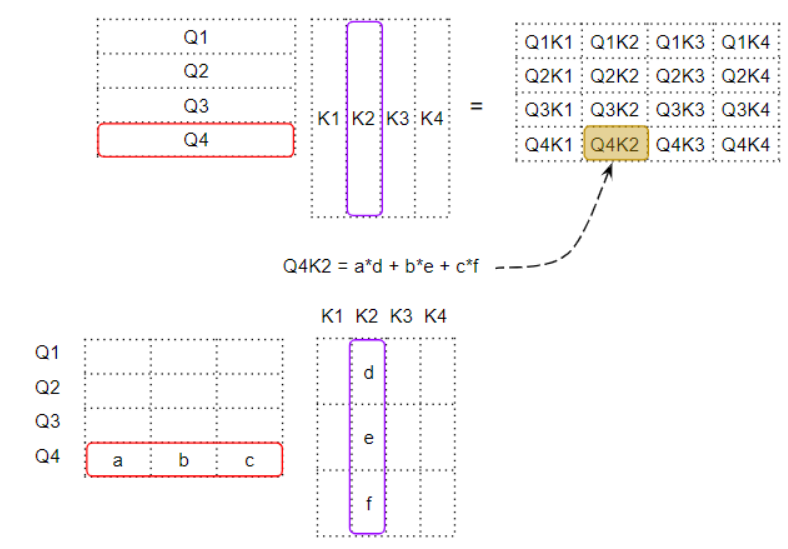
\includegraphics[width=0.9\textwidth]{figures/dot_prod_similarity.png}
	\caption{Dot Product of Query, Key and Value from here~\autocite{doshiTransformersExplainedVisually2021b}, depicting the resulting attention score.}
	\label{fig:dot_prod_similarity}
\end{figure}
This is excellently explained here~\autocite{doshiTransformersExplainedVisually2021b}:
\begin{itemize}
	\item If any two paired numbers, like `a' and `d'', are both positive or both negative then the product wil be positive. The product will
	      increase the summation.
	\item If one number is positive but the other negative then teh product will be negative. The product will decrease the summation.
	\item If the product is positive, the larger both numbers are, the more they contribute to the summation.
\end{itemize}
If the signs of the corresponding numbers in the two vectors are aligned, the final sum will be larger. This means a higher level of similarity,
or proximity between the two words.\\
For word vectors that are aligned the attention score is high, and vice versa for word vectors which are not aligned.
The ability to tune the parameter of the translations during training gives the model the ability to strengthen or weaken the alignment of the
words.
\bigbreak
As can be seen in \Cref{fig:attention_usage}, attention is used in three areas. The main concept and how attention works in the encoder has
been detailed. The other two areas are as follows.